\section*{Агентные модели}
\addcontentsline{toc}{section}{Агентные модели}
\subsection*{Подготовка к зачёту}
\addcontentsline{toc}{subsection}{Подготовка к зачёту}

\textbf{Задание:}\\
Реализовать модель подготовки к зачёту для одного студента.\\
Для подготовки к зачету дано N вопросов.\\
Студент использует следующую схему подготовки.\\
\begin{enumerate}[topsep=0pt,itemsep=-1ex,partopsep=1ex,parsep=1ex]
	\item Сначала он прорабатывает теоретический материал по очередному вопросу (и старается запомнить). Среднее время для этого по каждому вопросу одной тему колеблется в диапазоне от 30 до 40 минут (распределение равномерное).
	\item Затем студент по памяти воспроизводит материал изученного вопроса.
	\item Если материал не усвоен, то требуется повторение.
	\item После однократной повторной проработки вопроса студент переходит к следующему вопросу.
\end{enumerate}
Процесс продолжается до тех пор, пока не будут подготовлены все вопросы.\\
Степень усвоения изученного материала задается случайно (треугольное распределение от 5 до 100, мода - 60).\\

\textbf{Решение:}\\
Сначала необходимо создать популяцию вопросов. (Рисунок \ref{fig:questions1})
\begin{figure}[h]
	\centering 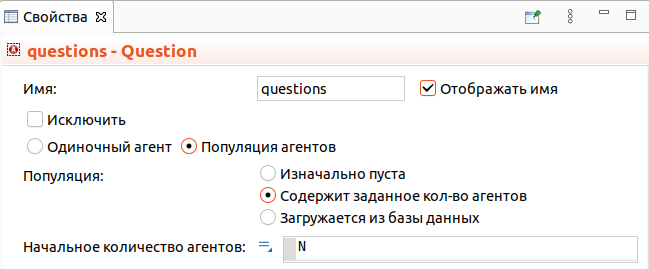
\includegraphics[scale=0.5]{questions1}
	\caption{Настройка популяции}
	\label{fig:questions1}
\end{figure}

\newpage

Каждый из вопросов имеет несколько состояний. (Рисунок \ref{fig:questions2})
\begin{figure}[h]
	\centering 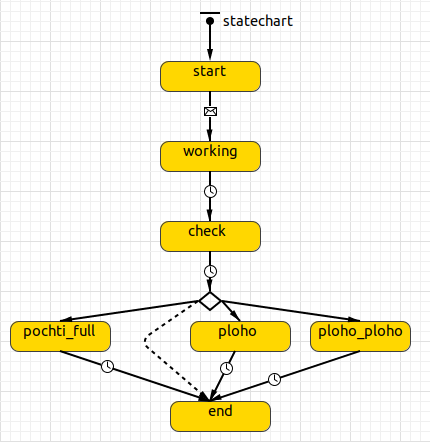
\includegraphics[scale=0.5]{questions2}
	\caption{Диаграмма состояний одного агента популяции}
	\label{fig:questions2}
\end{figure}

Переход между состояниями осуществляется в соответствии с правилами описанными в условии. Так как студент начинает подготовку вопроса при получении сообщения, то необходимо перед началом симуляции отправить сообщение о начале подготовки к первому вопросу. (Рисунок \ref{fig:questions3})
\begin{figure}[h]
	\centering 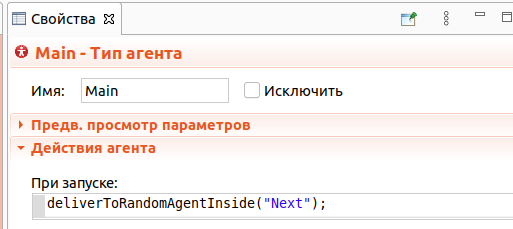
\includegraphics[scale=0.5]{questions3}
	\caption{Отправка сообщения первому агенту из популяции вопросов}
	\label{fig:questions3}
\end{figure}

\newpage

Если запустить симуляцию, то будет следующий результат. (Рисунок \ref{fig:questions4})
\begin{figure}[h]
	\centering 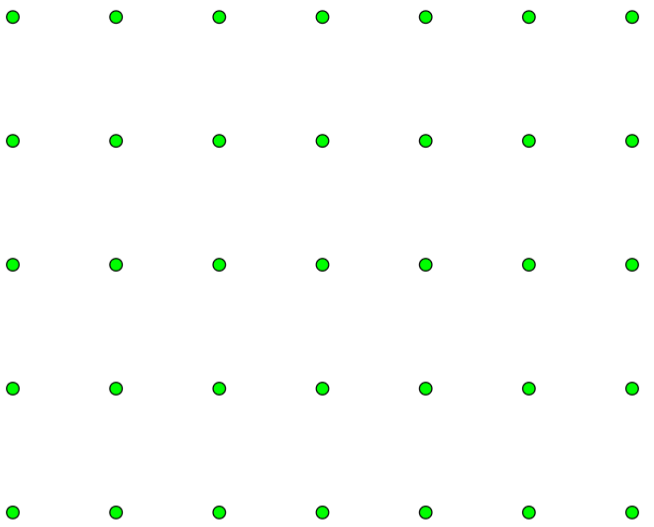
\includegraphics[scale=0.5]{questions4}
	\caption{Результат работы модели}
	\label{fig:questions4}
\end{figure}

Таким образом, была получена модель подготовки студента к зачёту.